\documentclass[border=3pt]{standalone}
% Preâmbulo compartilhado pelos diagramas TikZ da aula 7 de IHR (Emoção)
\usepackage[T1]{fontenc}
\usepackage[utf8]{inputenc}
\usepackage{lmodern}
\usepackage{amsmath}
\usepackage{xcolor}
\usepackage{tikz}
\usetikzlibrary{arrows.meta,angles,quotes,decorations.pathmorphing,decorations.pathreplacing,calc,
                positioning,shapes.geometric,shapes.misc,backgrounds,fit,
                math}

% Paleta (mesma dos SVGs originais)
% Paleta da disciplina de IHR: acento azul (#1A6FB5), cor de destaque do tema.
% (o nome "dblue" é mantido para não alterar todos os diagramas)
\definecolor{dblue}{HTML}{1A6FB5}
\definecolor{dorange}{HTML}{B3541E}
\definecolor{dgreen}{HTML}{4A7C59}
\definecolor{dred}{HTML}{9C4B4B}
\definecolor{dcream}{HTML}{F4F1EA}
\definecolor{dshade}{HTML}{DDD7C9}

% Função gaussiana (não normalizada por padrão de escala visual)
\pgfmathdeclarefunction{gauss}{3}{%
  \pgfmathparse{1/(#3*sqrt(2*pi))*exp(-((#1-#2)^2)/(2*#3^2))}%
}

% Estilos comuns (prefixo d... para não colidir com chaves internas do pgf)
\tikzset{
  >={Stealth[length=2mm]},
  dguide/.style={gray!55, dashed, line width=0.4pt},
  daxis/.style={gray!60, line width=0.7pt, ->},
  dbody/.style={fill=black!3, draw=black!80, line width=1pt},
  dacc/.style={draw=dblue, line width=1pt},
  dlbl/.style={black!55, font=\small},
  dsub/.style={black!45, font=\footnotesize},
  dstate/.style={circle, draw=black!80, fill=dcream, line width=1pt,
                 minimum size=17mm, font=\large, inner sep=1pt},
  dobs/.style={circle, draw=black!80, fill=dshade, line width=1pt,
               minimum size=14mm, font=\large, inner sep=1pt},
  dbox/.style={rounded corners=2pt, draw=black!80, fill=dcream, line width=1pt,
               align=center, inner sep=6pt},
  dop/.style={circle, draw=black!80, fill=white, line width=1pt,
              minimum size=6mm, inner sep=0pt, font=\small},
  dtrans/.style={->, dblue, line width=1pt},
  dmeas/.style={->, dorange, line width=1pt},
  dcurve/.style={line width=1pt, dblue},
  dcurveb/.style={line width=1.4pt, dorange},
}

\begin{document}
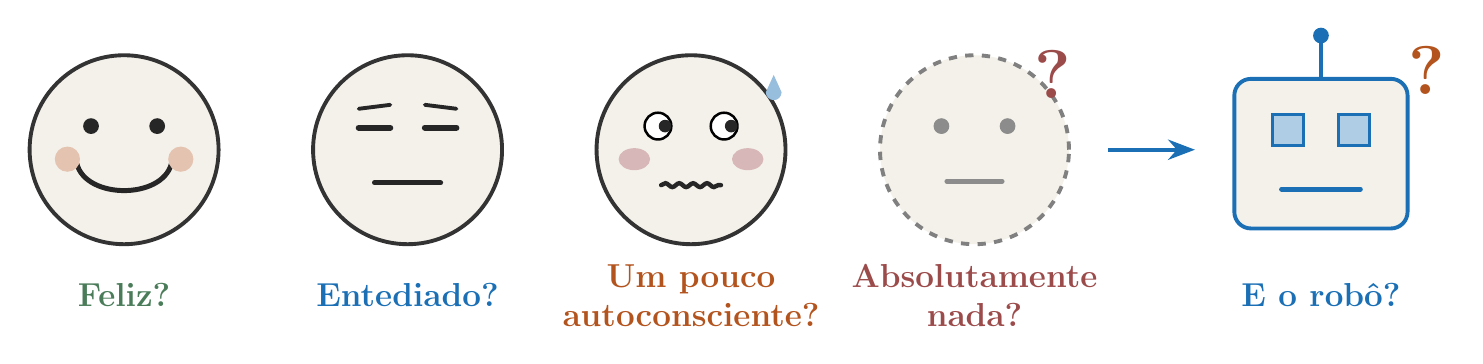
\begin{tikzpicture}[x=1cm,y=1cm]

  \tikzset{head/.style={circle, draw=black!80, fill=dcream, line width=1.4pt, minimum size=2.4cm},
           lab/.style={font=\large\bfseries, align=center}}

  % ---------- 1. Feliz ----------
  \begin{scope}[shift={(0,0)}]
    \node[head] at (0,0) {};
    \fill[black!85] (-0.42,0.3) circle (0.1) (0.42,0.3) circle (0.1);
    \draw[black!85, line width=1.8pt, line cap=round] (-0.6,-0.18) to[bend right=75] (0.6,-0.18);
    \fill[dorange!35] (-0.72,-0.12) circle (0.16) (0.72,-0.12) circle (0.16);
    \node[lab, dgreen] at (0,-1.85) {Feliz?};
  \end{scope}

  % ---------- 2. Entediado ----------
  \begin{scope}[shift={(3.6,0)}]
    \node[head] at (0,0) {};
    \draw[black!85, line width=2.2pt, line cap=round] (-0.62,0.28) -- (-0.22,0.28) (0.22,0.28) -- (0.62,0.28);
    \draw[black!85, line width=1.4pt, line cap=round] (-0.62,0.52) -- (-0.22,0.57) (0.62,0.52) -- (0.22,0.57);
    \draw[black!85, line width=1.8pt, line cap=round] (-0.42,-0.42) -- (0.42,-0.42);
    \node[lab, dblue] at (0,-1.85) {Entediado?};
  \end{scope}

  % ---------- 3. Autoconsciente ----------
  \begin{scope}[shift={(7.2,0)}]
    \node[head] at (0,0) {};
    \draw[fill=white, line width=0.9pt] (-0.42,0.3) circle (0.17) (0.42,0.3) circle (0.17);
    \fill[black!85] (-0.33,0.3) circle (0.08) (0.51,0.3) circle (0.08);
    \fill[dred!40] (-0.72,-0.12) ellipse (0.2 and 0.14) (0.72,-0.12) ellipse (0.2 and 0.14);
    \draw[black!85, line width=1.6pt, line cap=round, decorate, decoration={snake, amplitude=0.7pt, segment length=5pt}] (-0.38,-0.45) -- (0.38,-0.45);
    \fill[dblue!45] (1.05,0.95) -- ++(-0.1,-0.22) arc (180:360:0.1) -- cycle;
    \node[lab, dorange] at (0,-1.85) {Um pouco\\autoconsciente?};
  \end{scope}

  % ---------- 4. Nada? ----------
  \begin{scope}[shift={(10.8,0)}]
    \node[head, dashed, draw=black!50] at (0,0) {};
    \fill[black!45] (-0.42,0.3) circle (0.1) (0.42,0.3) circle (0.1);
    \draw[black!45, line width=1.8pt, line cap=round] (-0.35,-0.4) -- (0.35,-0.4);
    \node[dred, font=\Huge\bfseries] at (1.0,0.95) {?};
    \node[lab, dred] at (0,-1.85) {Absolutamente\\nada?};
  \end{scope}

  % ---------- seta e robô ----------
  \draw[dblue, line width=1.6pt, -{Stealth[length=3.4mm]}] (12.5,0) -- (13.6,0);
  \begin{scope}[shift={(15.2,0)}]
    \draw[line width=1.4pt, draw=dblue, fill=dcream, rounded corners=6pt] (-1.1,-1.0) rectangle (1.1,0.9);
    \draw[draw=dblue, line width=1.4pt] (0,0.9) -- (0,1.35); \fill[dblue] (0,1.45) circle (0.1);
    \fill[dblue!35, draw=dblue, line width=1pt] (-0.62,0.05) rectangle (-0.22,0.45) (0.22,0.05) rectangle (0.62,0.45);
    \draw[dblue, line width=1.8pt, line cap=round] (-0.5,-0.5) -- (0.5,-0.5);
    \node[dorange, font=\Huge\bfseries] at (1.35,1.0) {?};
    \node[lab, dblue] at (0,-1.85) {E o robô?};
  \end{scope}

\end{tikzpicture}
\end{document}
